\chapter{METODOLOGIA}

O desenvolvimento do projeto foi elaborado a partir de sessões tutoriais, laboratórios, criação de código e testes físicos na placa.

\section{Seções}
A maior parte das discussões e produções foram realizadas durante as sessões PBL, com toda a turma. Desde a leitura do problema até a elaboração de alguns trechos no Verilog, linguagem de descrição solicitada para o problema. Embora tenha exisitido uma dificuldade de adaptação aos conceitos da discplina nas primeiras sessões, a turma conseguiu redirecionar o foco para o que interessava inicialmente: criação de tabelas verdade, identificações de funções lógicas e desenvolvimento do código. Com esses dados, a criação do código de descrição no Quartus II (plataforma de desenvolvimento da Altera/Intel) ficou mais clara e concisa.

Sessões em laboratórios foram realizados para a noção física dos equipamentos e a interpretação de representação do código na placa. Esses laboratórios tiveram o suporte de roteiros que indicavam a utilização da plataforma Quartus, ensinando desde a criação de um projeto até a simulação dele.

\section{Recursos utilizados}
Em todo o processo de criação do protótipo , algumas ferramentas foram utilizadas como auxiliadoras no processo.

O Quartus II, em suas diversas versões, foi utilizado para a criação do projeto em Verilog \cite{weberarquitetura}. O programa conta com simuladores, apresentação de diagramas, determinação de pinos na placa, identificação de utilização de elementos lógicos, entre outros.

O Verilog é uma linguagem de descrição de hardware de fácil sintaxe e compreensão \cite{palnitkar2003verilog}, possibilitando seu uso para modelagem de sistemas eletrônicos físicos. Ele tem uma parte estruturtal, parecida com a sintaxe da linguagem de programação C, mas também conta com uma linguagem de mais baixo nível, a qual permite criação e relação de portas lógicas, que foram bastantes utilizadas nesse problema, com exceção de módulos básicos descrevendo elementos biestáveis.

Na parte de registro, o Overleaf foi utilizado como uma ferramenta que permite escrever em LateX, utilizando o modelo da ABNT disponibilizado no site do Módulo Integrador de Circuitos Digitais da UEFS. O site foi escolhido por ter uma ótima estruturação de escrita e permitir o desenvolvimento em grupo dentro da plataforma. Além do Overleaf, também para registros, o Trello foi utilizado como uma tabela de registro do que foi tratado nas sessões armazenando as ideias, fatos, questões e metas propostos pela metodologia PBL.

Fisicamente, o laboratório de hardware da UEFS (LEDS) foi utilizado como uma sala para a realização das sessões de laboratório, permitindo a realização dos testes nas placas, além da utilização de computadores como auxiliares na produção.

Os recursos bibliográficos estão apresentados na sessão de referência deste relatório.




\section{Descrição do código}
\section{Implementação física}

A implementação do código escrito em Verilog deve ser repassada para os circuitos integrados de lógica programável complexa (CPLD) para utilização do protótipo físico. 

Os CPLDs tem um funcionamento interno semelhante, mas mais complicados, aos integrados PAL e PLD. No CPLD existem vários sub-circuitos interconectados por uma matriz programável de interconexão global. Esses sub-circuitos recebem a nomenclatura de Logic Array Blocks (LABs) (Figura \ref{fig:diagramadeblocos}). Cada LAB contém blocos de I/O (entrada/saída), um circuito de expansão de termo produto e a quantidade de 4 a 16 macrocélulas. Cada macrocélula é estruturada com uma matriz AND conectada a uma matriz OR, para a implementação de soma de produtos, e flip-flops que, em alguns casos, são responsáveis pela realimentação de sinais na matriz AND \cite{CLPDarquitetura} O modelo utilizado foi o CPLD MAX II EPM240T100C5N.

Quando o código é ainda compilado no Quartus, uma série de informações acerca da implementação são geradas. No resumo do uso de recursos do Fitter, é possível ver todas essas informações. A partir do código apresentado neste relatório, temos as seguintes informações: 51/240 (21\%) elementos lógicos foram utilizados, todos no modo normal. Desses, no uso de elemento lógico por número de entradas LUT, 28 são de 4 entradas, 13 são de 3 entradas e 10 são de 2 entradas. Por fim, são utilizados 33 pinos, de 80 disponíveis (41\%).

\begin{figure}[!htb]
  \centering
    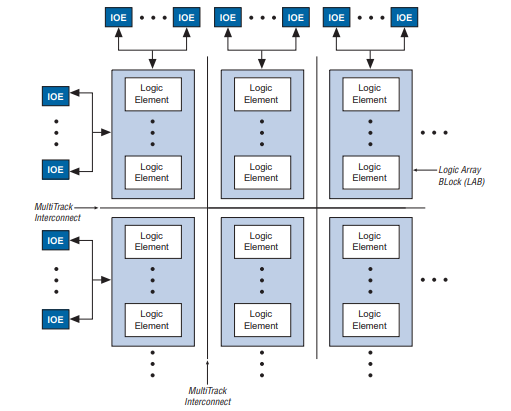
\includegraphics[width=0.7\textwidth]{imagens/diagrama.png}
  \caption{Diagrama de blocos do dispositivo MAX II}
  \label{fig:diagramadeblocos}
\end{figure}

\section{Teste e simulação}

Para realizar os testes físicos na placa, é recomendável realizar algumas simulações virtuais inicialmente, na tentativa de perceber os problemas antes de estarem conectadas na placa. Caso a simulação esteja correta, o ideal é que a aplicação física tenha um resultado adequado. 



